\documentclass[preview]{standalone}

\usepackage{amsmath}
\usepackage{amssymb}
\usepackage{stellar}
\usepackage{bettelini}
\usepackage{tikz}
\usepackage{fancybox}
\usepackage{makecell}

\usetikzlibrary{cd}

\hypersetup{
    colorlinks=true,
    linkcolor=black,
    urlcolor=blue,
    pdftitle={Biologia},
    pdfpagemode=FullScreen,
}

\begin{document}

\title{Biologia}
\id{biologia-enzimi-e-vie-metaboliche}
\genpage

\section{Reazioni tra enzimi e vie metaboliche}

\begin{snippetdefinition}{enzima-definition}{Enzima}
    Gli \textit{enzimi} sono dei catalizzatori per aumentare le tempistiche delle varie reazioni chimiche.
\end{snippetdefinition}

\begin{snippetdefinition}{metabolismo-definition}{Metabolismo}
    Il \textit{metabolismo} è l'insieme di tutte le reazioni chimiche nel corpo, catalizzate da un enzima.
\end{snippetdefinition}

\begin{snippet}{metabolismo-illustration-1}
    \begin{center}
        % https://tikzcd.yichuanshen.de/#N4Igdg9gJgpgziAXAbVABwnAlgFyxMJZABgBpiBdUkANwEMAbAVxiRAB12cYAPHYAIIBfEENLpMufIRQBGclVqMWbTtz7AAQiLETseAkQBMC6vWatEHLr34BhHeJAZ90ogGZTSi6psaAIjqKMFAA5vBEoABmAE4QALZIZCA4EEjy3ipWarbAMGAAXljxdAAEsiLUABYwdFBsOADuEDV1CLogsQnp1KlIJpmW1ur8+UUlpUaVIK31Vk0ttVDtTl2JiAN9iJ6DviN5hcVl7tOzDc2z7RRCQA
        \begin{tikzcd}
            \text{A} \arrow[r, "\text{enzima 1}", two heads] & \text{B} \arrow[r, "\text{enzima 2}", two heads] & \text{C} \arrow[r, "\text{enzima 3}", two heads] & \text{D}
        \end{tikzcd}
    \end{center}
\end{snippet}

\plain{Ogni reazione chimica ha il suo enzima.}

\begin{snippet}{metabolismo-illustration-2}
    \begin{center}
    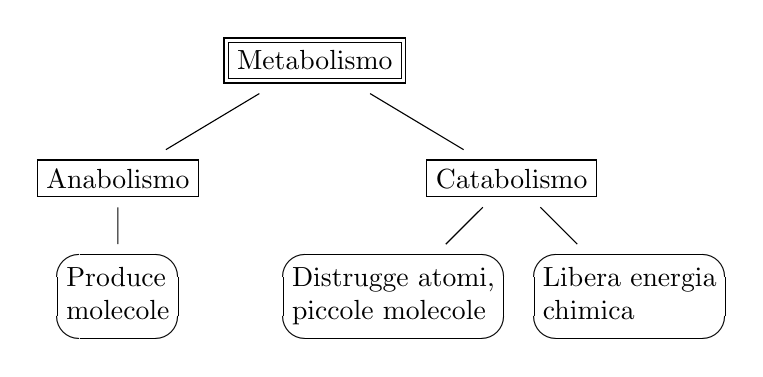
\begin{tikzpicture}[
        level 1/.style = {sibling distance = 5cm},
        level 2/.style = {sibling distance = 3cm},
    ]
    \node {\doublebox{Metabolismo}}
        child {
            node {\fbox{Anabolismo}}
            child {
                node {\ovalbox{\makecell[l]{Produce \\ molecole}}}
            }
        }
        child {
            node {\fbox{Catabolismo}}
            child {
                node {\ovalbox{\makecell[l]{Distrugge atomi, \\ piccole molecole}}}
            }
            child {
                node {\ovalbox{\makecell[l]{Libera energia \\ chimica}}}
            }
        };
    \end{tikzpicture}
    \end{center}
    \phantom{}
\end{snippet}

\plain{Il catabolismo produce ATP, mentre l'anabolismo serve per produrre materia.}

\begin{snippet}{catalisi-expl}
    \textbf{Catalisi:}
Una reazione chimica necessita che i reagenti si incontrino e si scontrino in una determinata maniera.
Questa è una questione probabilsitica, e in genere molto rara.
Per diminuire la velocità di reazione si possono utilizzare dei catalizzatori.
L'esempio più semplice di catalizzatore è la temperatura, siccome l'aumento della temperatura
aumenta la velocità di movimento delle molecole e, per cui, porta un aumento della probabilità di collisione.
Tuttavia, l'aumento della temperatura nel corpo non è sempre auspicabile, e vengono utilizzati
quindi degli anzimi come catalizzatori.
\end{snippet}

\includesnpt[width=65\%|src=/snippet/static/reactions-cat.png]{centered-img}

\begin{snippet}{2737aea4-3c4d-49e2-818f-07d5bdb69e83}
    Lo \textit{stato di transizione} è uno stato intermedio molto instabile.

    Gli enzimi offrono un posto dove i reagenti possono adagiarsi in maniera da collidere nella maniera
    corretta con gli altri reagenti.

    L'energia necessaria per arrivare lo stato di transizione (con enzima) è nettamente
    minore di quella per lo stato di transizione senza enzima.
    Questo è dato dal fatto che senza enzima vi saranno molti urti fra reagenti ma senza reazione.
    \[
        E_A = \textit{Energia di attivazione}
    \]
    Il posto dove vengono ospitati i reagenti nell'enzima si chiamano \textit{siti attivi}.
\end{snippet}

\includesnpt[width=65\%|src=/snippet/static/enzym-cat.png]{centered-img}

\plain{L'enzima trascina i reagenti sullo stato di transizione.}

\includesnpt[width=60\%|src=/snippet/static/energy-reaction.png]{centered-img}

\section{Inibitori enzimatici}

\begin{snippetdefinition}{inibitore-enzimatico-definition}{Inibitore enzimatico}
    Con il termine \textit{inibitore enzimatico} si indica una molecola in grado di instaurare un legame chimico con un enzima, diminuendone così l'attività. 
\end{snippetdefinition}

\begin{snippet}{inibitore-expl1}
    È possibile che una molecola (inibitore), simile al reagente, occupi il 
posto nell'enzima dedicato al reagente. Questo blocca l'enzima e, per cui, la reazione chimica.
Gli inibitori vengono prodotti quando è necessario ridurre il numero reazioni chimiche
(Es. per feedback negativo, farmaco).
\end{snippet}

\begin{snippet}{tipi-inibitore}
    Gli inibitori possono essere due tipi:
    \begin{itemize}
        \item \textbf{competitivo:} occupa il posto del reagente nello spazio ativo;
        \item \textbf{non competitivo:} deforma lo spazio attivo con un legame in un altra posizione.
    \end{itemize}

    Entrambi i tipi di inibitori possono essere \textit{reversibili} o \textit{irreversibili}.
\end{snippet}

\end{document}